  
%\title{Title page with logo}
%----------------------------------------------------------------------------------------
%	PACKAGES AND OTHER DOCUMENT CONFIGURATIONS
%----------------------------------------------------------------------------------------

\documentclass[12pt a4paper]{article}
\usepackage[english]{babel}
\usepackage{amsmath}
\usepackage[margin=25mm]{geometry}
\usepackage{tabularx}
\usepackage{graphicx}
\usepackage{titlesec}
\usepackage{float}
\usepackage{chngcntr}
\usepackage{caption}
\usepackage{listings}
\usepackage{subcaption}
\usepackage{csquotes}
\usepackage{hyperref}
\hypersetup{
    colorlinks,
    citecolor=black,
    filecolor=black,
    linkcolor=black,
    urlcolor=black
}
\usepackage[citestyle=authoryear-icomp ,bibstyle=numeric]{biblatex}
\addbibresource{lib.bib}



\begin{document}

\begin{titlepage}

\newcommand{\HRule}{\rule{\linewidth}{0.5mm}} % Defines a new command for the horizontal lines, change thickness here

\center % Center everything on the page
 
%----------------------------------------------------------------------------------------
%	HEADING SECTIONS
%----------------------------------------------------------------------------------------

\textsc{\LARGE University of St. Andrews}\\[1.5cm] % Name of your university/college
\textsc{\Large CS4099}\\[0.5cm] % Major heading such as course name
\textsc{\large Senior Honours Project}\\[0.5cm] % Minor heading such as course title

%----------------------------------------------------------------------------------------
%	TITLE SECTION
%----------------------------------------------------------------------------------------

\HRule \\[0.4cm]
{ \large \bfseries Automatic Identification of Cell Motion, Splitting, and Death in a 4D Dataset\\[0.4cm]} % Title of your document
\HRule \\[1.5cm]
 
%----------------------------------------------------------------------------------------
%	AUTHOR SECTION
%----------------------------------------------------------------------------------------

\begin{minipage}{0.4\textwidth}
\begin{flushleft} \large
\emph{Author:}\\
Gareth Cairns % Your name
\end{flushleft}
\end{minipage}
~
\begin{minipage}{0.4\textwidth}
\begin{flushright} \large
\emph{Supervisor:} \\
Dr.~David Harris-Birtill% Supervisor's Name
\end{flushright}
\end{minipage}\\[2cm]

% If you don't want a supervisor, uncomment the two lines below and remove the section above
%\Large \emph{Author:}\\
%John \textsc{Smith}\\[3cm] % Your name

%----------------------------------------------------------------------------------------
%	DATE SECTION
%----------------------------------------------------------------------------------------

{\large April 2019}\\[2cm] % Date, change the \today to a set date if you want to be precise

%----------------------------------------------------------------------------------------
%	LOGO SECTION
%----------------------------------------------------------------------------------------

\includegraphics[height=4cm]{logo.png}\\ % Include a department/university logo - this will require the graphicx package
 
%----------------------------------------------------------------------------------------

\vfill % Fill the rest of the page with whitespace

\end{titlepage}

% \null\vspace{\fill}
% \begin{abstract}
% Abstract
% \end{abstract}
% \vspace{\fill}
% \newpage

% Title Page done -----------------------------------------------------------------------------------------------------------

\begin{abstract}
The aim of this project is to provide a program to be used by the Biology Department of
the University of St. Andrews. The program will be used to monitor cell movement, cell
splitting and cell death as they develop in the embryo; this enables researchers to understand
the processes as cells start to form in organs. Biologists interested in tracking cell motion,
splitting, and death, currently use a time consuming manual method of tracking the cells using
bespoke software, pinpointing all cells’ location in 3D space at a given time, the time this takes
to conduct limits the number of experiments they can conduct. This project seeks to automate
this cell tracking process using computational methods, therefore enabling researchers to
perform more detailed experiments and free up researchers’ time.
\end{abstract}
\section*{Declaration}
I declare that the material submitted for assessment is my own work except where credit is explicitly given to others by citation or acknowledgement. This work was performed during the current academic year except where otherwise stated. The main text of this project report is 11,806 words long, including project specification and plan. In submitting this project report to the University of St Andrews, I give permission for it to be made available for use in accordance with the regulations of the University Library. I also give permission for the report to be made available on the Web, for this work to be used in research within the University of St Andrews, and for any software to be released on an open source basis. I retain the copyright in this work, and ownership of any resulting intellectual property

\newpage
\tableofcontents
\newpage

\section{Introduction}
The tracking and analysis of cells is an important field of research within the Biology Department of the University of St. Andrews. Analysis of cell motion, splitting and death are instrumental in understanding the process of organ development, and the effects of medicines on the processes of cell motion, splitting and death. The commonly used process for tracking cells in research come from manual methods; this entails manually selecting each cell for each frame captured, with large datasets, this leads to the researchers having to down-sample the data-set size by only taking samples for example, every 5 frames instead of frame by frame. Not all cells can be tracked manually as it would take too long to perform the individual tracking, this means that not all cells are tracked, and potentially, information is lost to the researchers. This process is labour-intensive and slow, requiring a considerable amount of a researcher's time which could be better spent processing data rather than gathering. To take less of a researcher's time, this project aims to automate the cell tracking process, providing quicker results for researchers all the while gaining more data, with a comparable accuracy. The final product of this project will be able to identify cells from within a three dimensional Z-stack of TIF images of cell microscopy (Figure \ref{fig:z-stack}), and track them over a duration of time, given by the length of the input set, by linking cells found in Z Stacks between frames. This process will create trails of motion for each cell over time, noting times of cell death and of division. The tracked cell data will be output into a format readable by the software used by the Biology department. Tracked cell data will be compared to manually tracked information so that an accuracy metric can be given, allowing a researcher to decide if the system accuracy is acceptable, given the time savings from this automated method.
\begin{figure}
    \centering
    \includegraphics[width=0.55\textwidth]{Images/Z-Stack.png}
    \caption{A Z-Stack of 2D Cell Microscopy images, representing a 3D scan of the cells, used as the basis for 3D tracking.}
    \label{fig:z-stack}
\end{figure}
The objectives of this project are as follows:
\begin{itemize}
    \item To create a literature review on the current state-of-the-art in the field of cell tracking and cell biology to aid in furthering the field.
    \item To create an end-to-end project to perform automated tracking of cells over time in a 3D space. This must be able to detect cells in the 3D space of a Z-Track of images, and track these cells over time. The data output by the tracking must be in a format usable by Dr.~Bischoff.
    \item To capture critical interesting moments within the cell data such as cell death and mitosis.
\end{itemize}

The primary objective of this project is to create an end-to-end product which could be used by the Biology Department and Dr.~Bischoff, to aid in the process of tracking cells, creating an automated workflow to capture the important data such as the location of a cell over time.

The secondary objective would be to detect when a cell has split in the process of mitosis, or has died during tracking. These are important steps in the growth of an organism, therefore, capturing these events could be important for research.
A tertiary objective would be to discern more details about the cell over time, such as, what cells are its' parents, does it split, and what is the lineage of this cell.

\newpage
\section{Literature Review}
The following section will be the result of my research into this field of Cell Tracking. I will explore the current state of the art so to ensure that my project can help progress the current standard of work in the field of Cell Tracking in Drosophila.
    \subsection{Cell Biology Background}
% Morphogenesis
Morphogenesis is the process which forms the organs within an organism, it also dictates the overall shape of the organism. 
% Movement in morphogenesis
During morphogenesis, cells can undergo mitosis, die, or move in patterns to form the structure of organs. Mitosis is the process of nuclear division in cells that occurs when a parent cell divides into two identical daughter cells (\cite{mitosis}). These cells move together in groups but it is important to know the behaviour of individuals rather than the group as this is what directs morphogenesis. The movement of the cells is an essential function in the cellular system; in multi-cellular organisms such as Drosophila, cell movement is the driving force for morphogenesis and preserves homoeostasis(\cite{miura_2005}).

% knowing how drugs affect cell movement in morphogenesis is important to know
Tracking cells in this process enables automated analysis of the duration of single phases of the cell life cycle, and thus the identification of cell cultures that show abnormal behaviour. Tracking can also be chosen to investigate the affects of certain drugs on cellular proteins which can play a part in cell movement, and can even be used to recognise the development of cancer cells (\cite{harder_mora-bermúdez_godinez_ellenberg_eils_rohr_2006}).

% Too many photos for manual tracking
Automated tracking tools can be very important for a Biologist as often the manual tracking of 4D data-sets can be very highly labour intensive and may detract from more important aspects of their research such as analysis. Automation in this tracking process can allow for Biologists to prioritise their analysis more heavily and could work to the benefit of speeding up research in the cell biology and morphogenesis fields.
% Number of Ways to track
    \subsection{Current Tracking Technology}
    Cell tracking is a field with many tools available right now, whether this be automated or manual. The biology department of the University of St. Andrews is using .smd files in tandem with the SIMI Biocell software for manually tracking cell locations. (\cite{bischoff_cseresnyes_2009})
    
    Some current automated solutions are successful in their niche but may not be suited to all cell data. This can be caused by specific tuning to a certain organism's cells, which may be of a different size to what is required in another data set.  The aim of this project is to aid in the automated tracking for cells within Drosophila, most tools aren't built specifically for this organism and cannot provide the same level of accuracy that bespoke software can offer.
    
    The current cell trackers can often struggle with more complex tracking events such as mitosis and death (\cite{huh-et-al}). This causes the researchers using the tracked data to have to manually check for errors due to these issues, meaning that the time benefits of an automated system become negated.
    
    Another struggle of current tools for cell tracking is their inability to detect cells when the images aren't clear enough. If the image has too much noise, is too bright, or has low contrast then the tools can struggle to detect a cell, which means that a cell could fail to track. Image processing techniques are used to improve the clarity of these samples allowing them to be tracked. 
    
    Temporal snapshotting frequency, how often the cells are captured in photos, must be low due to the photo-damage that can be caused from exposing the cells to harsh light too often. This can cause cell death which may skew the results of the tracking.(\cite{Awasthi})
    \subsection{Automated Tracking}
    To track a cell, a multi-stage process must take place which will identify the cells, then track them throughout the sequence of images (\cite{MEIJERING2012183}). To identify the cells, a technique called Image Segmentation can be used; this will process the image to give regions where it finds a cell. Cell-Linking is the second part of this process where using algorithmic techniques, cells in different parts of the spatio-temporal sequence are found to be the same cell, having potentially either moved or slightly changed shape. This second step is what allows tracking to truly take place as you can then map the movements and find the velocity of the cells that you are interested in for the morphogenesis process. Cell-linking can provide us with a lot of challenges due to the nature of the moving cells; some cells can be attributed easily to the wrong cell in the next frame, skewing the results greatly.
        \subsubsection{Image Segmentation}
        The Image Segmentation step has multiple different approaches you can take to achieve the same end goal of isolating every cell within the image. Sometimes multiple approaches need to be taken to gather the greatest accuracy and in this section, a discussion of some of the more popular methods will be shown.
        
        % Thresholding
        Thresholding is a method almost universally used in segmentation of images (\cite{miura_2005}). Thresholding is used to discern an object of interest from the background of the image. This can be done by setting a threshold brightness or colour value which contrasts with the background and categorising each pixel in the frame as either background or object pixels, discerning if a pixel is closer to the threshold of the background colour or intensity (\cite{MEIJERING2012183}). Thresholding is a basic method and has multiple cases where its use may fail; these reasons include: severe noise in the the image, and photo-bleaching from fluorescence photography, poor contrast within the images. A method to remove background noise before the thresholding step is to apply a Gaussian blur, smoothing out points of noise to match the background, this gives us clearer results (\cite{opencv}).
        
        % Template Matching
        The template matching approach to image segmentation is sometimes used for cell detection. This method requires at least some human interaction to identify a template cell in the image initially. This template cell is used to scan the image for similar looking regions which the model will determine as cells if the template matches the sample closely enough (\cite{MEIJERING2012183}).. This method has the downside of being unable to cope with any abnormal cells, as they would not match the template and the system would not detect these cells as close enough to the template image. Cells undergoing mitosis can also be difficult for this approach to detect and so template matching is usually only used in conjunction with other methods to improve its accuracy. Some models for template matching use an evolving template which is updated and generalised using information from the image of what a cell in this data set generally looks like. 
        
        % Gradient Methods
        While pattern matching methods are commonly used in Biological research, the "gradient method" is used in broader areas of tracking. This method is more robust than the template matching methods. The gradient method is more equipped to deal with cell deformation as it relies on image differentials to detect cells instead of a rigid template which must be adhered to.
        
        % Active Contouring
        Active contouring is a method employed by some current segmentation and tracking systems. This approach will simultaneously detect edges and be able to track movement. A contour is formed around the cells to outline the borders of the cell, this is a deformable model which can handle cell deformation and even cells touching each other(\cite{li-et-al}). Cell-Cell contact can be dealt with using repulsive forces on the edges of the cells which are touching, meaning that the cell boundaries will never overlap (\cite{li-et-al}).
        
        % Watershed transformations
        Watershed transformations are a method of segmentation commonly used in conjunction with thresholding, specifically to help separate touching cells, which may be detected as one large cell using other segmentation methods. The watershed transformation method completely separates images into regions and delimiting contours which can be used to split the regions (\cite{Awasthi}), however, this method can easily lead to over-segmentation (\cite{chen_zhou_wong_2006}) and so can be the most useful when used in conjunction with other methods of segmentation, to give the most accurate results.
        
        \subsubsection{Cell Tracking}
        Cell tracking is used to monitor movement of cells within the observed organism, it also should be able to track mitosis events in the cell life cycle, creating a link between mother and daughter cells, in turn creating a lineage associated to the tracked cell (\cite{thirusittampalam}). Automated tracking of cells is faced with a number of challenges increasing the difficulty of accurate tracking, these challenges include: having to use low contrast images in which cell locations may be hard to discern, cells changing shape over time, cell divisions occurring and cells interacting with each other such as collisions (\cite{thirusittampalam}).
        
        % Gaussian Masks in Thresholding
        % Nearest Neighbour approaches
        The nearest neighbour approaching to linking cells between frames is simple to understand and implement. This method will find every cell at frame t and try to match it to whatever cell is closest to the initial cell in frame t+1. This approach is simple to implement but is prone to errors as the density of cells in the sample image increases, another cell may move closer to the initial position than the moving cell may settle (\cite{DORN2008497}). A slightly modified version of the nearest neighbour approach is global nearest neighbour which will search through all the pairings of cells between frames t and t+1 to find the arrangement with the lowest average displacement between the centre points of all cell pairs (\cite{DORN2008497})., however, this does not consider the effect of cell motion, meaning that often times the results of this method can be sub-par, especially when the movement of cells exceeds half the mean distance between the cells. Some systems will use a probabilistic model to analyse multiple frames before and after before linking the cells from frame to frame (\cite{DORN2008497}). 
        
        % Feature Matching in nearest neighbour 
        Nearest neighbour can also be improved by changing the definition of nearest. By default, nearest means least displacement, however, it can be changed to be the closest in likeness by the use of pattern matching. These characteristics can be used in conjunction with the displacements of the cells (\cite{handetal}). Pattern matching can be used in this way to link cells between frames which appear the most alike, whether that is in shape, size or overall appearance. It can be beneficial to use pattern matching with nearest neighbour as it then allows for errors due to cell movement being avoided which is useful due to the nature of the cells that this project aims to track as cells tend to move in a certain direction (\cite{miura_2005}). The density problem of nearest neighbour can be solved using pattern matching as it is easier to track if a certain cell has moved. An issue with this approach is any time where the cell morphology changes, this can result in incorrect tracking results (\cite{handetal}, \cite{thirusittampalam}), morphology changes tend to happen at the time a cell is undergoing mitosis (\cite{Hamahashi2005}) which will make the goal of tracking cell events such as mitosis considerably more difficult.
        
        % Model Evaluation
        % Active Contouring
        
        No one method of cell tracking is fully satisfies the requirements of the system this project aims to build and so the system must include a combination of some of these methods to make this cell tracking system one of the most accurate available.
        \subsubsection{Mitosis Detection}
        Mitosis events are possible to detect due to a few facts that there are some physical characteristics which change, such as, shape, texture, and colour, and thus can be detected by our detection system (\cite{irshad2013automated}). The overall brightness of a cell increases as mitosis takes place, this allows us to discern a cell undergoing mitotic changes from the average cells (\cite{huh-et-al}). From here, a probabilistic model is used to guess if a birth event takes place, and if so, which frame of the cell data.
        Another method to detect a mitotic event is to use reverse cell tracking, you can find a mitosis event when two tracked cells converge onto a location and only one cell is found, this indicates that one cell has split into two, capturing the event of mitosis.
        
        The morphology of a cell can be used to detect if mitosis has or will take place by monitoring the following morphological features: area, roundness, elongation, perimeter and equivalent spherical perimeter. These features have been highlighted by the detection software by \cite{irshad2013automated} as key parameters to detect mitosis.
        
        
% More details of advantages and disadvantages of how other people have done it. What accuracies are involved? More methodologies and case studies. Doesn't give what is the state of the art. Give metrics. 
% ========================================== REQUIREMENTS =======================================
\newpage
\section{System Requirements Specification}
\subsection{Objectives}
Listed in this section are the agreed upon objectives for the final version of this software project, a successful attempt at the problem will fulfil these requirements.
\subsubsection{Primary}
The following list details the primary objectives of development in this project.
\begin{enumerate}
  \item Generate a Literature review to explore the current state of the art in this field. Image processing techniques will be reviewed along with specifically cell image processing to gather an understanding on how to approach the project.
  \item Identify cells in the data-set images.
  \item Track individual cells over time throughout the data-set.
\end{enumerate}


\subsubsection{Secondary}
The following list of requirements shows the secondary objectives set for this practical.

\begin{enumerate}
    \item Output cell tracking data in a format readable by the Biology Department's manual cell tracking software, SIMI Biocell as a .smd file.
    \item Include cell death and cell splitting events into tracked data and a cell lineage.
    \item Analyse and compare the program output to human-labelled cell tracking data to gather an accuracy metric.
\end{enumerate}

\subsubsection{Tertiary}
The following list of system requirements outline the tertiary objectives for this project moving forward.
\begin{enumerate}
    \item Implement Automatic labelling of interesting events in the output file.
\end{enumerate}
\newpage
\section{Software Engineering Process}
Throughout this project I have used the Agile development method, creating iterative design improvements to the product. I initially focused on the context survey, as to best research approaches to tackle the problem of cell detection and tracking, then I moved onto the software development, focusing on achieving a minimum viable product which had the ability to detect cells within images and gather information such as size from that cell.

After achieving the minimum viable product, I focused on creating numerous iterations on a weekly sprint schedule, as to align with the weekly supervision meetings throughout the development process. During development, I used the Agile development method model to split large pieces of functionality into small, achievable chunks as to build the system. This process used physical post-it notes on a pin-board as to keep track of progress, and what needed to be done within the project. For the writing of this report I am using Trello boards which are an online equivalent to a pin-board, where issues can be tracked and functionality to be completed can be checked upon. An example Trello board can be seen in Figure \ref{fig:Trello}.

Before development started, I realised that Agile development was the correct direction to follow as it led to quick tangible results while models such as Waterfall may have been too slow, causing for less rapid development, causing delays in this project.
\begin{figure}
    \centering
    \includegraphics[width=0.8\textwidth]{Images/SH-Trello.png}
    \caption{A Trello Board Example for Report Writing}
    \label{fig:Trello}
\end{figure}
\subsection{Software Requirements}
The software requirements for this project are as follows in Tables \ref{table:softwareReq} and \ref{table:libReq}, outlining the software which must be installed along with the libraries for the external features. 
\begin{table}[H]
    \centering%
    \caption{Software Requirements for Project}
    %TC:group tabular 1 1
    \begin{tabular}{p{\dimexpr0.25\textwidth-2\tabcolsep-\arrayrulewidth\relax}|
                    p{\dimexpr0.75\textwidth-2\tabcolsep-\arrayrulewidth\relax}
                  }
        \hline Requirement & Requirement Description \\ \hline \hline
        Python 3.6 & Required to launch the program and load external libraries.\\ \hline
        Tkinter & A Python extension used to create and display graphical user interfaces, to allow for an intuitive method of input to the program. \\ \hline
        Unix Operating System & A Unix based operating system such as Linux or MacOS allows for the implementation of this project to work as intended.
        \label{table:softwareReq}
    \end{tabular}
\end{table}

\begin{table}[H]
    \centering%
    \caption{Library Requirements for Project}
    %TC:group tabular 1 1
    \begin{tabular}{p{\dimexpr0.25\textwidth-2\tabcolsep-\arrayrulewidth\relax}|
                    p{\dimexpr0.37\textwidth-2\tabcolsep-\arrayrulewidth\relax}|
                    p{\dimexpr0.37\textwidth-2\tabcolsep-\arrayrulewidth\relax}
                  }
        \hline Requirement & Requirement Description & Use Case \\ \hline \hline
        Numpy & A mathematics library, granting the ability to create matrices. &  Used to create a "footprint" matrix to define the region for a cell to be found in.\\ \hline
        Scipy & A library with pre-built functions for common tasks in scientific computing & Using the Gaussian filter algorithm on images to aid in the detection process along with tools for measuring areas of found cells in the detection system.\\ \hline
        Pandas & Data Analysis library supplying data structures used by common statistical tool & DataFrame object used as a the data structure for clustering algorithm.\\ \hline
        Matplotlib & Data plotting library in Python &  Used to generate all visually plotted outputs of data.\\ \hline
        Python-CV2 & Library supplying support for image reading and manipulation. & Used to load in .TIF images used by the Biology Department. \\ \hline
        Sci-kit Image & Provides an array of image analysis and manipulation methods.  & Used to segment images using watershed segmentation and thresholding.\\ \hline
        Sci-kit Learn & A library with a variety of Machine Learning methods included, built to work with Pandas data structures & Used for the DBSCAN clustering method within the cell detection phase of the pipeline. 
        \label{table:libReq}
    \end{tabular}
\end{table}

% ===============================================================================================
\newpage
\section{Ethics}
This project uses data from the University of St Andrews School of Biology, the data consists of cell microscopy images of fruit flies. As these images are of the cells of an invertebrate species there are no animal rights ethics concerns involved in the project. No human data is involved in this project and therefore no special ethical considerations must be made for the research or implementation of this project.

% ====================================== DESIGN ================================================
\section{Design}
\subsection{Project Pipeline}
The finished project will use a graphical user interface so that a user can find it easy to operate the system I build. The GUI must be the starting point of any pipeline I want to create, where an image set can be chosen from a directory. This chosen image set should be able to be tracked or preview the tracking settings so that the system can be fine tuned. An image set should also be able to be made into a short video that demonstrates the tracking system over time which will be output in a common format so that the video can be played on many devices. 

If a user chooses to use the tracking functionality of the program, the resulting output should be a .smd file used by the Biology department, so that the file format matches the in-place workflow for the researchers. The .smd file should be readable by the software currently used and should contain useful information such as the locations of a cell overtime. The smd file must contain a minimal amount of unnecessary information such as incorrectly identified cells as to keep the file size to a minimum, therefore optimising the performance of their later analysis of the tracked cell information.

The structure and data flow of such a pipeline is shown in Figure \ref{fig:sysPipe}.
    \begin{figure}
        \centering
        \includegraphics[width=0.8\linewidth]{Images/SystemPipeline.png}
        \caption{Overview of the System Pipeline for this Cell Tracking Software.}
        \label{fig:sysPipe}
    \end{figure}
\subsection{Cell Detection}
The cell detection system should be able to take in a single image from the cell microscopy dataset and return a list of cells and their locations to provide either a preview of the cell detection system or alternatively for the later tracking stages in the system pipeline.

An image should be loaded from a file using Python, from a folder specified by the user for tracking, or an individually chosen image for detection previewing. The image must be prepared for the segmentation process, removing any image noise or flaws within the image and ensuring that the image is in a format which the segmentation algorithm can interpret and analyse, to ensure that the results of the segmentation process can be optimal and correct. 

A segmentation algorithm must be chosen so that the image of cells can be interpreted as a collection of individual discrete regions (cells). This algorithm must have a high accuracy in finding the correct regions of the image in which the cells reside.

The segmented regions of the image must be analysable so that we can discern the centre point of the cells and the overall area, this area will be used to filter out the smaller and larger cells found by the algorithm to allow the user to track particular size ranges of cells, removing information tracking of irrelevant cells. A system to be in place to remove cells such as blood cells from tracking, as they often only appear for one frame, causing false matches between cells. After these processes, a list of cells should be returned for the image, either forming part of the cell data for a Z-stack or populating a list of cells to display as the output of a preview.

This pipeline is visualised in  Figure \ref{fig:cellDetPipeline}. The output of this pipeline is to be a list of cells, the cells in this list will provide the basis for the tracking algorithm to be later used on the dataset.
\begin{figure}
    \centering
    \includegraphics[width=\linewidth]{Images/CellDetectionPipeline.png}
    \caption{Cell Detection Pipeline}
    \label{fig:cellDetPipeline}
\end{figure}
\subsection{Video Output}
As mentioned in the Cell Detection Pipeline, it should be possible to generate a preview of the cell detection settings over time on a certain level of the Z-stack, loading a data-set into the program, and outputting a video file of the mp4 format. 

This video output should be used as a good indication of how well the detection is working over time, and will also serve in giving a useful visualisation of the overall process.

\begin{figure}
    \centering
    \includegraphics[width=\linewidth]{Images/VideoGeneration.png}
    \caption{Video Generation Pipeline}
    \label{fig:vidGenPipe}
\end{figure}
\subsection{Cell Tracking}
To track cells we must link them from frame to frame of our cell detection system. As stated in the Cell Detection design section of this report, each time a Z-stack is ran through the cell detection system, we will receive a list of found cells in the Z-stack. Running the tracking will require cell data for each Z-stack in the data-set, ensuring we have a complete set of data for the location of the cells over time.

Each cell should be linking using a matching algorithm with a corresponding cell in the previous frame. If a cell cannot be matched it should be then marked as a new cell, coming from a mitotic event in the system. Each cell should have a history attached to it detailing previous locations, when it was born, what cell it divided from (if applicable), and how many children cells it created.

An important stage in this process is knowing when a mitotic event happened, a process must be in place to identify the event. From the context survey, it has been seen that backtracking through the dataset is an effective method of detecting a mitosis event. An algorithm will be in place to backtrack through the dataset and check if two cells converge on a certain location at a given time, with the previous frame having only one cell in that place. Although this may not lead to perfect accuracy, it will give a good approximation of the mitotic activity with the data. 

One algorithm mentioned within research during the context survey to match cells between two frames is the nearest neighbour algorithm, this would an ideal algorithm for this process due to the fact that it is relatively quick to compute, which is the overall goal of this project. 

To keep our computational time low in the tracking process, we must ensure that all the cells we are tracking at a given time are cells worth tracking, for example, we do not want to be tracking a cell which we have detected as dead, or having moved outside of the frame. In these cases, we should store the information of these cells but not have them in the list of cells we are currently keeping track of; this process will greatly reduce the number of cells we must match per frame in the processing of our cell data.


\begin{figure}
    \centering
    \includegraphics[width=\linewidth]{Images/TrackingPipeline.png}
    \caption{Cell Tracking Pipeline}
    \label{fig:cellTrackPipeline}
\end{figure}
\subsubsection{SMD File Output}
Our tracked cell data must be output in the format of the .smd file type as to be used by the researchers in the Biology department. This means I must follow the format defined in the .smd specification which was given to Dr.~Bischoff by the developers of the SIMI Biocell application. Following this specification, I can supply a compatible file which can be used by Dr.~Bischoff and his team. Figure \ref{fig:smdSpec} shows the specification including necessary header information for the file. Another point of reference for this file format comes from one of Dr.~Bischoff's manually tracked .smd files, which shows the format of a tracked cell as is shown in Figure \ref{fig:smdExample}.
\begin{figure}
    \centering
    \includegraphics[width=0.8\linewidth]{Images/smdFormat.png}
    \caption{The .smd File Format Specification}
    \label{fig:smdSpec}
\end{figure}

\begin{figure}
    \centering
    \includegraphics[width=0.4\textwidth]{Images/SMDExample.png}
    \caption{An Example of Manually Tracked .smd File Format.}
    \label{fig:smdExample}
\end{figure}
\subsection{Cell Lineage and Death}
The tracked cells within my system must have a method of storing information on their current alive status and contain information about their cell lineage. This entails cells having the ability to store which other cells in the system are their offspring. 

To store this information, the most logical system is a binary tree which will contain the family relation, as each cell can have at most one parent and will have two daughters when it splits. Storing the relations in this format will result in a tree structure showing the lineage of a cell.

Upon instruction from Dr.~Bischoff, it is recommended to encode the death of a cell simply within the location information that a cell contains within the .smd specification. Location data of a file in a .smd file can contain a comment for researchers to mark in interesting moments in the cell life-cycle (Figure \ref{fig:smdSpec} shows this). In the last tracked location of any given cell, we can include a comment indicating that a cell has died at this point. 
\subsection{User Interface}
The user interface for this project must be a in the form of  GUI which allows for the selection of a directory of images to analyse. There should be fields in which to fine tune the settings of the segmentation process, allowing for adjustments to be made, allowing the correct cells to be located.

The GUI should allow the user to preview their segmentation settings, create a video preview, and also initiate the tracking pipeline. 

The GUI should allow the user to select an image at any depth of the Z-Stack over any period of time.

The user should be able to preview the settings of the segmentation algorithm. This would entail the ability for an image to be shown from within the GUI, and the ability to select a particular image to check.

From here, the user should be able to initiate the tracking process from within the GUI, resulting in the output file.

\newpage

\section{Implementation}
The following section details the process of implementing the design decisions formed within the previous section of this report. Included in this section will be the novel solutions used to solve the problems set by the requirements of this program. Most design decisions made are to the benefit of functionality, however, some were made to ensure that the speed of the computation remained feasible whilst giving the best possible results. 
\subsection{Cell Detection}
To detect cells within 3D space from a Z-stack of cell microscopy images, the pipeline detailed in Figure \ref{fig:cellDetPipeline} must be implemented, the following subsections explain the details of the implementation of this pipeline for the project, using python and various Python libraries to gather information on a cell's location in 3D space at any one given time.

To implement this pipeline, I used two separate approaches to detect cells; the first approach was to load and segment each image separately, as to detect each cell lying on each Z-stack level, then linking all these found cells in the Z-stack to create a single list of cells for that one point in time. This approach has the limitation of some cells appearing in more than one particular Z-stack level, leaving us with the task of detecting whether a cell detected has already been detected or if it is newly discovered, a solution to this problem is discussed later in this subsection. 
The second approach is to use the function supplied by the Numpy library, called dstack. This is an algorithm which can join the data of multiple pre-processed images as to gain an array representing a 3D model of the Z-stack (\cite{oliphant2006guide}). This allows for segmentation to take place on a 3D dataset rather than an set of 2D images, providing us with the information for the detected cells without the computationally complex and possibly inaccurate methods for detecting cells within multiple images. The outputs in Figures \ref{fig:filtSize} and \ref{fig:prefilt} show the 2D approach to segmentation, while Figure \ref{fig:3DCells} shows the output of the 3D stack of images used as input to our segmentation system.

\subsubsection{Pre-Processing}
To prepare the cell images for the segmentation stage of cell detection, we follow the process shown in Figure \ref{fig:prePro}. This pre-processing step in our process is multi-staged in its implementation, using multiple image processing functions to help achieve the best possible results in the segmentation process.

\begin{figure}
    \centering
    \includegraphics[width=\textwidth]{Images/Detection/PreProcess.png}
    \caption{Pre-Processing Pipeline}
    \label{fig:prePro}
\end{figure}

The first step in pre-processing our images is to load in the images we intend to segment. For previewing our settings, this involves loading a single image of the user's selection which will be sent through the rest of the pre-processing pipeline. For our tracking, we must load in all of the images representing one frame of the 3D cell microscopy data set and processing them individually.

The function we use to alter our input image is to apply a Gaussian blur to the image, this helps to remove noise from our input image which can cause over segmentation within the watershed segmentation process later (\cite{gauch1999image}). This process can be seen in Figures \ref{fig:blurred} where we use Figure \ref{fig:before} as our input. This process keeps the overall detail of the image while removing any static or noise.
\begin{figure}
  \centering
  \begin{minipage}[b]{0.4\textwidth}
    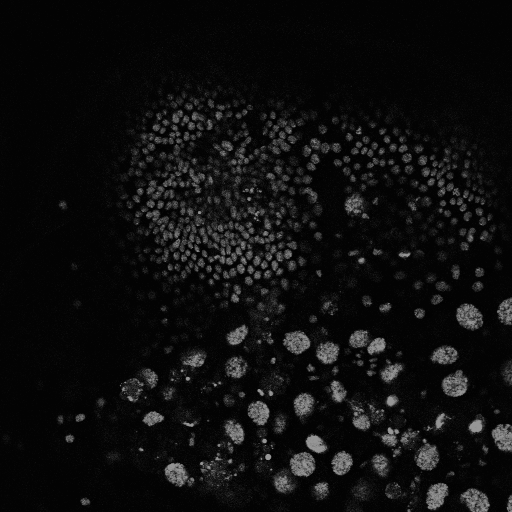
\includegraphics[width=\textwidth]{Images/Detection/1Before.png}
    \caption{Loaded Image Before Processing}
    \label{fig:before}
  \end{minipage}
  \hfill
  \begin{minipage}[b]{0.4\textwidth}
    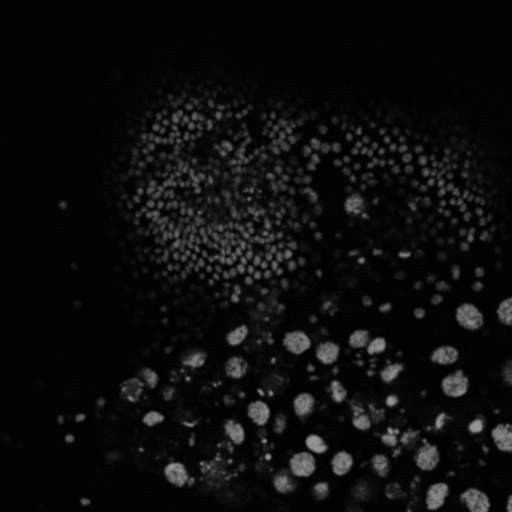
\includegraphics[width=\textwidth]{Images/Detection/2Gaussian.png}
    \caption{Gaussian Blur applied to Cell Microscopy Image}
    \label{fig:blurred}
  \end{minipage}
\end{figure}
Using our Gaussian blurred image (Figure \ref{fig:blurred}), we must calculate our threshold for which we computationally decide which pixels in the input image are classified as the background or the foreground/subject based on the brightness values of our input image. The process of thresholding I use for this project is known as Otsu's threshold, which is able to compute threshold values of brightness on a local scale (\cite{vala2013review}, \cite{kittler1985threshold}). This allows us to retain more detail on shapes within our input image (Figure \ref{fig:otsuTresh}) as this method checks for large changes in brightness within particular regions, which it interprets as the background and foreground brightness values. A comparison of thresholding using an absolute value of brightness as background and foreground and using an adaptive Otsu threshold is shown in Figures \ref{fig:sub-abs} and \ref{fig:sub-otsu}.



\begin{figure}
    \centering
    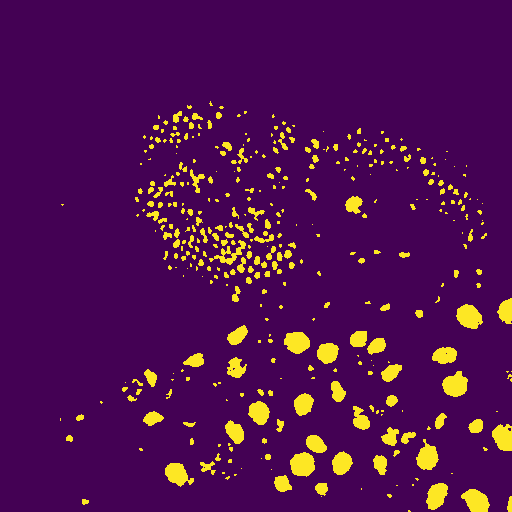
\includegraphics[width=0.4\linewidth]{Images/Detection/3Otsus.png}
    \caption{Otsu's Thresholding/Binarisation Technique on Cell Microscopy Image}
    \label{fig:otsuTresh}
\end{figure}

\begin{figure}
  \centering
  \begin{subfigure}{.5\textwidth}
  \centering
  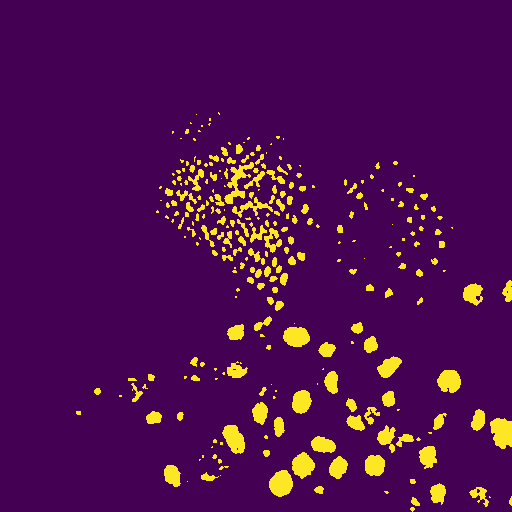
\includegraphics[width=0.6\linewidth]{Images/Detection/3Thresh.png}
  \caption{Absolute Thresholding}
  \label{fig:sub-abs}
\end{subfigure}%
\begin{subfigure}{.5\textwidth}
  \centering
  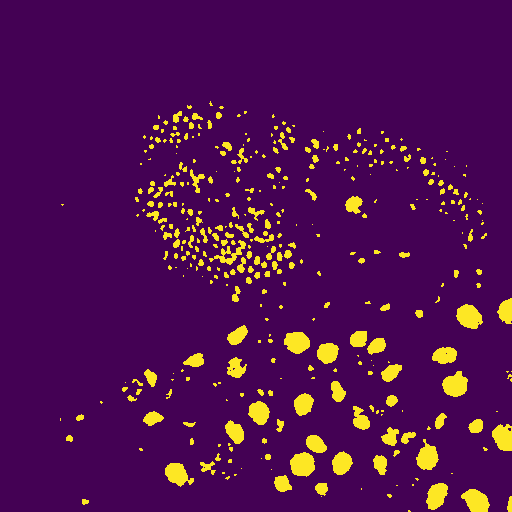
\includegraphics[width=0.6\linewidth]{Images/Detection/3Otsus.png}
  \caption{Otsu Thresholding}
  \label{fig:sub-otsu}
\end{subfigure}
\label{fig:comp}
  \caption{Comparison of Otsu Threshold vs Absolute Value Thresholding between two different image samples.}
\end{figure}
The user can specify a multiplier to be applied to the Otsu threshold values calculated by the system, as to allow them to fine tune the system to detect cells or regions of the image which may not be correctly detected with the default Otsu values. The effects of setting these values manually can be seen in Figures \ref{fig:sub-high} and \ref{fig:sub-low} where in the low multiplier, the cells are not correctly separated by the thresholder, creating a large mass of all the bright cells, and where the high multiplier can dramatically increase separation between cells ensuring that the cells do not overlap or touch for our segmentation step. Each dataset will need slightly different threshold parameters to perform optimally, so allowing the users to set these values is a useful feature.
\begin{figure}
  \centering
  \begin{subfigure}{.5\textwidth}
  \centering
  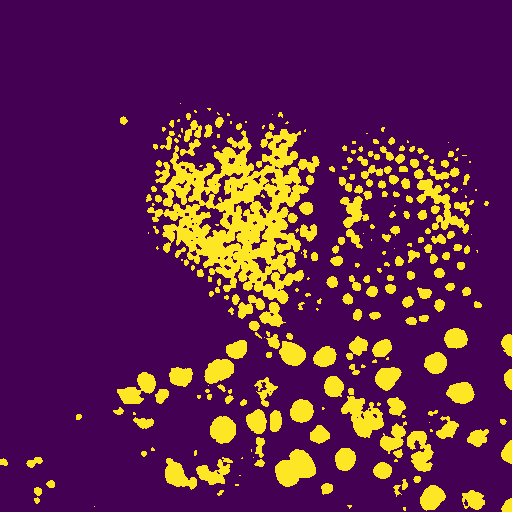
\includegraphics[width=0.9\linewidth]{Images/Detection/3LowTresh.png}
  \caption{Low Threshold - A Threshold of $0.5 \times Otsu Threshold$}
  \label{fig:sub-low}
\end{subfigure}%
\begin{subfigure}{.5\textwidth}
  \centering
  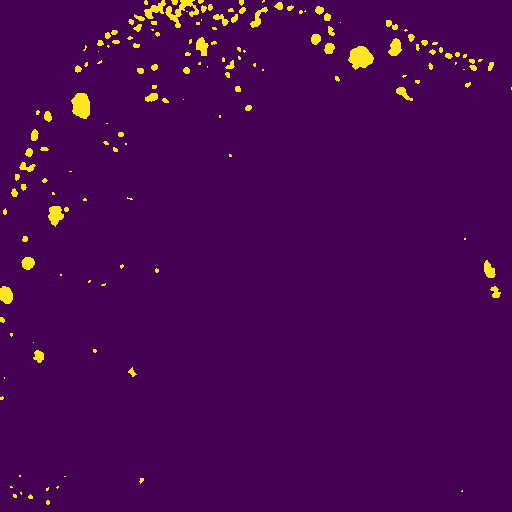
\includegraphics[width=0.9\linewidth]{Images/Detection/3HighTresh.png}
  \caption{High Threshold - A Threshold of $2 \times Otsu Threshold$}
  \label{fig:sub-high}
\end{subfigure}
  \caption{Comparison of a High and Low Thresholding Output in input images.}
  \label{fig:lowvshigh}
\end{figure}
The next step in the pre-processing phase, is to apply the binary closing function to the output of \ref{fig:otsuTresh}. Binary closing is a method to fill in small holes within the binary image output of the thresholding step of pre-processing (\cite{chen1995recursive}). This process is used to ensure that the shapes found through the threshold step are continuous shapes as opposed to regions with holes which may cause the watershed segmentation algorithm to over-segment.

\begin{figure}
    \centering
    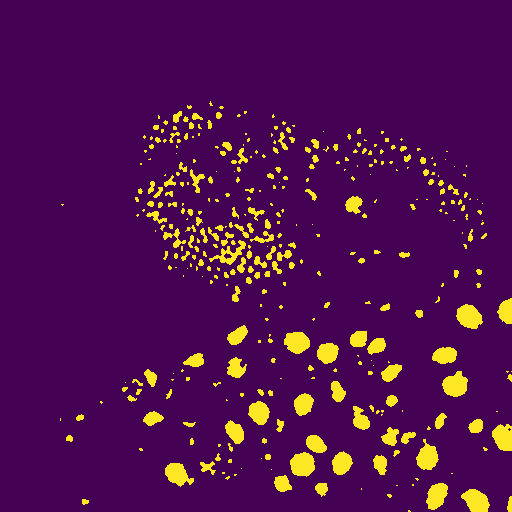
\includegraphics[width=0.6\linewidth]{Images/Detection/4BinClosing.png}
    \caption{Result of Binary Closing Processing of an Image, with Figure \ref{fig:otsuTresh} as the Input}
    \label{fig:bin_closing}
\end{figure}

The final step in the pre-processing phase is to apply a filter on the discovered regions of the image in which we detect a cell shape. This filter is called clear borders and will remove any regions of our binary image in direct contact with the borders of the image frame (\cite{clear}). This process ensures that we will not try to detect cells which may only be half in the frame of the image.
\begin{figure}
    \centering
    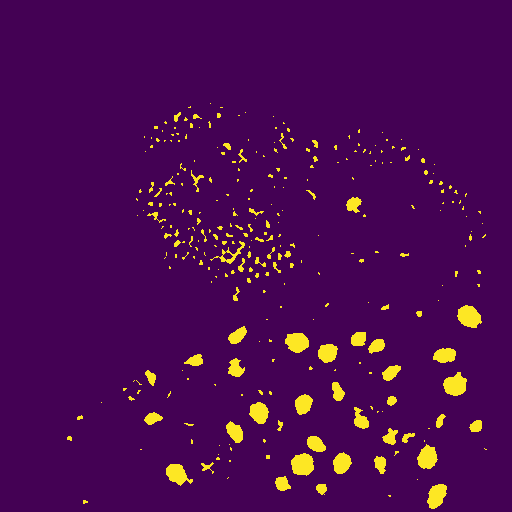
\includegraphics[width=0.4\textwidth]{Images/Detection/6ClearedBorder.png}
    \caption{Result of Clearing Objects touching the border of the image, with Figure \ref{fig:bin_closing} as the Input.}
    \label{fig:clearBorder}
\end{figure}

\subsubsection{Watershed Segmentation}
For this project, I opted to use watershed segmentation due to its ability to detect items which are very close to each other or touching. Due to the dense cluster of cells within our dataset, this was discerned to be a perfect use case for the watershed method (\cite{matlab&simulink}).

Watershed segmentation requires more pre-processing than simply thresholding and clearing the borders of the image. We must perform more computations for the watershed algorithm to function. This includes the calculation of a distance transform which is used to map how far each pixel within a shape is to the edge of the shape (\cite{rao2002modification}), this results in an output like in Figure \ref{fig:distanceTransform} which shows the detected blobs as blurred regions instead of solid shapes. This is to assist in the next stage of the watershed process which is to find the local maxima of each shape. This is essentially the centroid points of the segmented shapes as due to how the distance transform is performed, the brightest areas of a shape are at the centre (\cite{rao2002modification}). Finding the local maxima is a process to find the brightest regions individual sections of the image (\cite{gauch1999image}) which is seen within Figure \ref{fig:localMaxima}. 

\begin{figure}
    \centering
    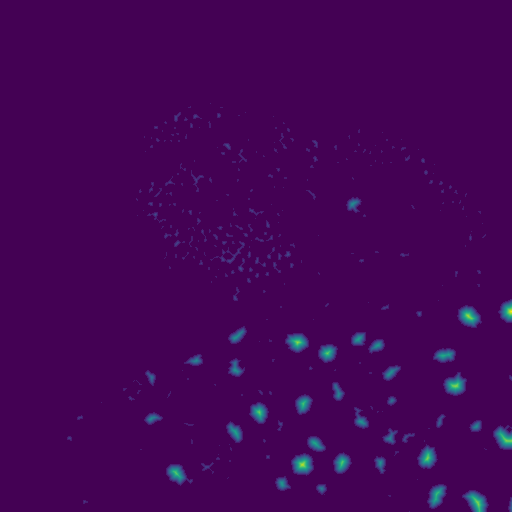
\includegraphics[width=0.4\textwidth]{Images/Detection/7DistTransform.png}
    \caption{Distance Transformation for Watershed Segmentation with Figure \ref{fig:clearBorder}'s cleared borders as the input.}
    \label{fig:distanceTransform}
\end{figure}

\begin{figure}
    \centering
    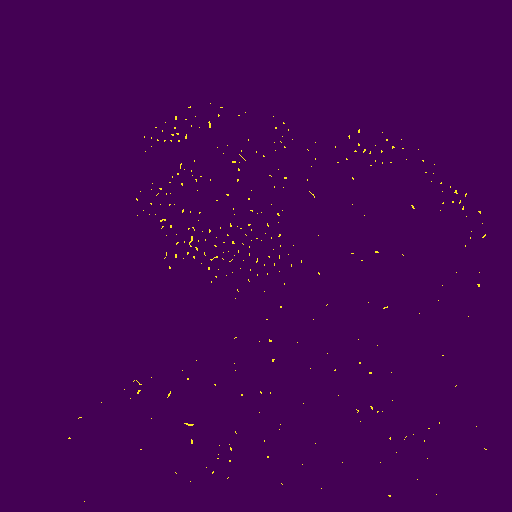
\includegraphics[width=0.4\linewidth]{Images/Detection/8LocalMaxi.png}
    \caption{Finding Local Maxima from the Distance Transformation Image seen in Figure \ref{fig:distanceTransform}}
    \label{fig:localMaxima}
\end{figure}

When the local maxima are found, we use this information along with the distance transform as input to the watershed segmentation algorithm. This algorithm is used to find the points at which there is a separation between two objects, defining their boundaries (\cite{beucher1992morphological}). These boundaries are found by using catchment basins which are seen in Figure \ref{fig:catchment}, which act as 3D surfaces, into which the "watershed" happens, effectively separating regions by "flooding" them, which is simply increasing the threshold at which we separate the connected entities, and define their borders at the watershed line, also seen in Figure \ref{fig:catchment}. The catchment basins are computed from the distance transforms, where each point in a shape is given a distance value which acts as a value of a 3D surface's height, from which we can use the flooding technique to separate entities.

\begin{figure}
    \centering
    \includegraphics[width=0.4\textwidth]{Images/Detection/mathWorks-Watershed.png}
    \caption{3D Catchment Basis for Watershed (\cite{matlab&simulink})}
    \label{fig:catchment}
\end{figure}

A parameter used in watershed segmentation is the footprint, in the local maxima point finding. This parameter sets the region in which the algorithm will look for a maxima point. Setting this parameter allows the user to specify the size of region they expect their cells to fall in to. A comparison of small and large footprint is shown in Figure \ref{fig:footprint}. In this example, we can see that setting the footprint value too high means that we struggle to capture all the details and cells within our input image; this may lead to under segmentation.

\begin{figure}
  \centering
  \begin{subfigure}{.5\textwidth}
  \centering
  \includegraphics[width=0.9\linewidth]{Footprint/5x5.png}
  \caption{A 5x5 footprint in which we check for local maxima.}
  \label{fig:sub-5}
\end{subfigure}%
\begin{subfigure}{.5\textwidth}
  \centering
  \includegraphics[width=0.9\linewidth]{Footprint/10x10.png}
  \caption{A 10x10 footprint in which we check for local maxima.}
  \label{fig:sub-10}
\end{subfigure}
  \caption{A comparison in cell detection in the same image for segmentation processes containing different footprint sizes to check for local maxima.}
  \label{fig:footprint}
\end{figure}

When these parameters are set, we can then perform the watershed segmentation on our input image or image stack. The output of this process is shown in Figure \ref{fig:watershed}, where each segmented region is given its own colour as shown by the colour bar. These labelled regions are input for the next stage in our cell detection process, filtering of cells.

\begin{figure}
    \centering
    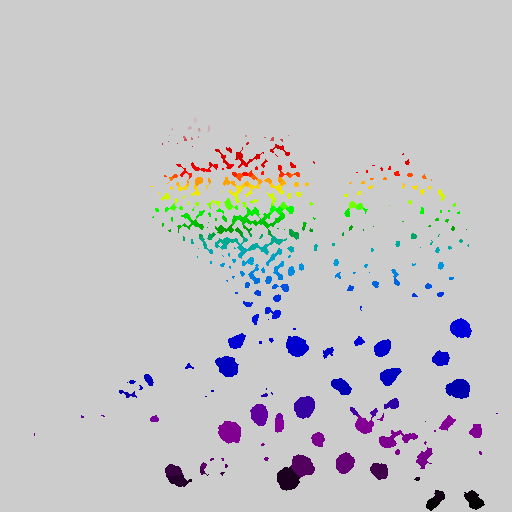
\includegraphics[width=0.8\textwidth]{Images/Detection/9Watershed.png}
    \caption{Output of Watershed Segmentation Process on the input image. The colours shown represent the label attributed to a region, with each label being given a different colour.}
    \label{fig:watershed}
\end{figure}
\subsubsection{Filtering of Cells}
Detected cells within the watershed process are assigned labels which denote which pixels belong to which segmented object; this allows us to gain information on the labelled objects such as their area covered using the Scikit-Image function measure.regionprops() which automatically discerns the area covered by each label in the output of the watershed segmentation. The user can set a limit for what they discern to be a cell in the system with an upper and lower boundary to the size of detected regions in the GUI. The regions which are below the minimum size threshold or above the maximum are discerned to be noise and are removed from the output data. This acts as a filter for cells which we do not want to track within the system. This process can be seen within Figures \ref{fig:prefilt} and \ref{fig:filtSize} which show the detected cells before and after filtering, showing that more "noisy" data points are removed from the data set. This may remove some cells that are not noise data points, so allowing the users to set their thresholds can help minimise this effect.
\begin{figure}
    \centering
    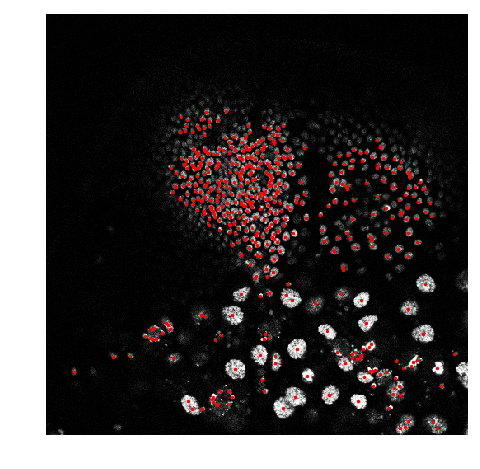
\includegraphics[width=0.4\textwidth]{Images/Detection/10PreFilt.png}
    \caption{Cells tracked through watershed method, before filtering of cells occurs with their centroid points marked using red dots.}
    \label{fig:prefilt}
\end{figure}

\begin{figure}
    \centering
    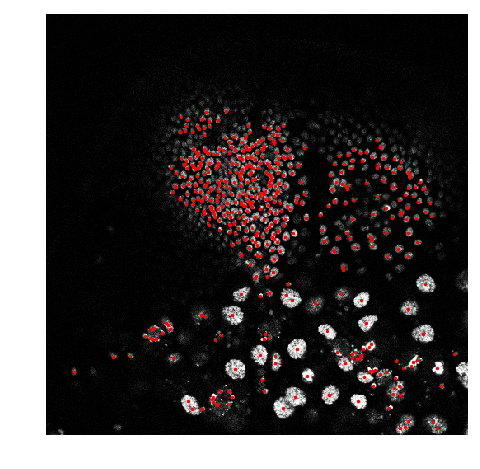
\includegraphics[width=0.4\textwidth]{Images/Detection/11Filtered.png}
    \caption{Detected cells filtered by the area they cover, within a lower and upper area threshold.}
    \label{fig:filtSize}
\end{figure}




\subsubsection{Cluster Detection}
Once the cells have been detected within the dataset, it is then important to restrict the number of cells found, as the cells detected are usually outside of the core cluster that the researchers find important. This can be seen in Figure \ref{fig:filtSize}, where outside of the core cluster of cells, some outliers can be seen  amongst the cells in the periphery of the image. These cells are not tracked within the manually tracked data, and therefore, I have decided to filter them out as to leave the outputs consistent with the researcher's desired results. This also has another useful outcome, being that the less cells we detect, the quicker our tracking system will be as less comparisons need to be made between cell locations.

The algorithm I have chosen to implement for this cluster detection is known as Density-Based Spatial Clustering Applications with Noise or DBSCAN. DBSCAN aims to detect the core points of a cluster (\cite{ester1996density}). A core point is defined as a point in which a specified number of other points lie within a specified radius of that point (\cite{borah2004improved},\cite{ester1996density}). Two parameters define this clustering system, first of which being $\epsilon$ which denotes the radius in which you look for the existence of other points, and the minimum number of points within the search radius to define a point as a core cluster point. Within the DBSCAN algorithm, a data point can be described as a core cluster point, a border point or an outlier point (\cite{borah2004improved}). A border point is a point in the dataset which is not a core point but lies within the radius of a core point, and an outlier point is one which is neither a core point or lies within one's radius.

To classify each point within the dataset, the algorithm will randomly select a data point, check if the requirements hold for it to be a core point, and if so, label all points within its radius as a border point unless that point is already defined as core. This process continues until all points in the dataset have been checked under the constraint of being a core cluster point. All points not defined as border or core are then set to being outliers.

For each detected cell within my segmentation output, I check for the property of it being core. This process allows me to remove the outlier cells from the dataset, regarding them as noise within the system. This allows us to deal with more amounts of data for the next step in the system pipeline, tracking the detected cells.

\begin{figure}
    \centering
    \includegraphics[width=0.7\textwidth]{Images/Detection/dbscan-HE.png}
    \caption{A Visual Representation of the DBSCAN algorithm (\cite{He2014}). Where A0..An are the core cluster cells discovered by the algorithm, B0..Bn are cluster border cells, and N is the outlier cell found by the algorithm.}
    \label{fig:heDBSCAN}
\end{figure}
\begin{figure}
    \centering
    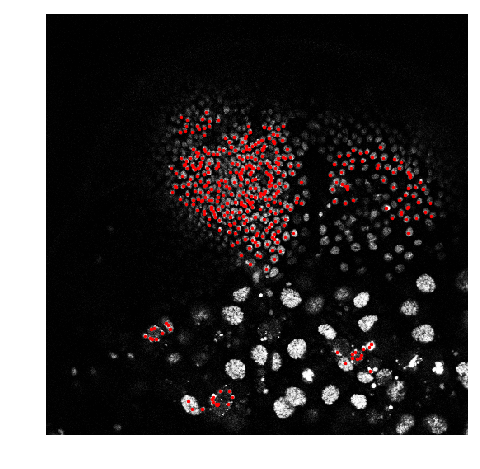
\includegraphics[width=0.7\linewidth]{Images/Detection/12ClusterFiltered.png}
    \caption{Detected cells after filtering by using DBSCAN to detect the dense clusters of cells, removing outliers.}
    \label{fig:my_label}
\end{figure}
\subsubsection{Cell Representation}
To correctly represent a cell within this project, I implemented a class which could be used to compute and represent the data that is needed within the SMD file format.

For this task, I defined the Cell class within Python which creates a Cell object with the following attributes: an identifier (cell name), daughter cells (left and right), a list of Points in 3D over time, and an attribute denoting if a cell is within the core cluster, a border cell, or is an outlier. The data stored for each cell found within the system is enough to create a useful output for the SMD file format as specified in Figure \ref{fig:smdSpec}.


\subsection{Multi-threading of Cell Detection}
Due to this project's focus on speed of computation, I implemented the process of cell detection and all its component parts, down to cluster detection, in a thread-safe fashion, allowing for multi-threading of the process which can increase the overall processing speed by utilising more of the CPU in a computer (\cite{sodan2010parallelism}). 
To allow for this multi-threading, the system will group the input images into their respective Z-stacks. This allows us to process the relevant images together at the same time as each group of images is segmented independently from each other. Due to there being no overlap in data or data-structures used in each case of segmentation, we can process these groups of images within their own threads using the multiprocessing library provided by python. This library allows us to "pool" tasks together, in this case, I defined each group of images as a task to be processed and when a thread is ready to process some data, it will select a task from the pool to compute. 

These tasks can be taken from the pool out of order, however, the Pool.map() function returns the results of every task into a list that retains the order, which is crucial for the tracking process later in the pipeline as a cell must be linked from one time to another.

Multithreading of this nature can give the large speed increases in computation (\cite{sodan2010parallelism}), due to the fact that processing this data in sequence will take $n \times computationTime$ where n is the number of jobs to finish, while with multi-threading, we could in-theory achieve $(n/ threads) \times computationTime$ which can offer us a significant boost in processing speed on multi-core computer systems. 
\subsection{Video Output}
During development I found that it may be beneficial to the users of my application to have an output to preview segmentation over time instead of in a single photo.
For this reason, I created the video output feature of my application. This feature will segment all images in a dataset on a certain level of the Z-stack, this will act as a slice of the dataset overtime. Each image runs through the segmentation process to output an image in the Output folder created by the application.
These images are saved to the disk as png files, these files are then loaded back into the system by the CV2 library in Python.

CV2 offers a VideoWriter object which I use to create a video output of the cell images by defining each segmented image of the Z-stack as a frame in a video. Each video is output as the height and width of the output images from the segmentation process.
The video we have generated using the CV2 library can then be output to the Output directory storing the intermediate images in the process as a .MP4 video. This video format was chosen due to its ability to be viewed on a wide range of devices, such as mobiles or laptops, therefore allowing for the outputs to be more easily output between researchers and vetted to ensure that the segmentation process is achieving what they had initially aimed to achieve in the cell detection process.
\subsection{Cell Tracking}
The tracking of cells within the 3D Cell microscopy data-sets is a fundamentally difficult problem due to the fact that there are multiple targets that need tracked, these targets can cross paths in the data which can lead to target-association problems such as incorrect linking of cells throughout time (\cite{li2002detection}).

The method of cell linking I have chosen to implement is Nearest Neighbour target matching. I chose this algorithm due to its relatively low computational cost compared to some other approaches. 
Nearest Neighbour tracking is a naive approach to matching targets over time. Each cell or target detected will be attempted to be matched to a cell or target at the next time step, to match the cells together, we computer the distance of every cell in t + 1 to the cell in t and, if the minimum distance is less than a defined radius, we match the cell at t to the cell at t + 1 with the lowest error. We cannot have a cell in t + 1 attributed to more than one cell in t, therefore we shall remove the closest cell from the list of cells that can then be tracked to. This ensures that each cell will be matched to the nearest possible cell available in the list. Unfortunately this method relies on a correct ordering of points as to ensure that cells are not mismatched to cells in t + 1 as another cell in t may be closer to a cell in t + 1. Computing this is very resource intensive as we must compute every single match for all cells, when trying to produce reasonably quick results, this is not a viable option, so the approach of finding the best of the remaining cells is what we are constrained to. A visualisation of how a cell is matched between frames can be seen in  Figure \ref{fig:nn} which depicts the selection process used to match cells, the nearest cell will be the one chosen by the algorithm as the cell's match in the next frame.

\begin{figure}
    \centering
    \includegraphics[width=0.6\textwidth]{Images/Tracking/GraphicalNN.png}
    \caption{Graphical representation of the nearest−neighbour (NN) method for finding the "best" match for the target (\cite{DNN}). In this example, A1 is found to be the nearest neighbour as the distance D1 is the smallest of the computed distances between the chosen point and neighbours}
    \label{fig:nn}
\end{figure}
Ideally, this approach to ensure that all cells are correctly matched using the Global Nearest Neighbour algorithm will be used in later iterations of this project where the results gained may be more true to the output of the manually tracked data. The Global Nearest Neighbour algorithm aims to find the minimal error within tracking between times t and t + 1 (\cite{konstantinova2003study}), finding the lowest total displacement of cells from one frame to another. For another attempt at this project, I would recommend Global Nearest Neighbour tracking being implemented.
\subsubsection{Tracking Output}
When the tracking stage has finished, we generate a list of cells found over time, these cells will contain information on their locations over time. These cells are required to be output as smd files. To get the output of cells, we sort the list of cells by the time that they first appeared in the dataset. This allows the smd file to be in chronological order of cell discovery which makes manual pruning of the automated tracked cells easier on a user. 

As discussed before in the Cell Representation section, the tracked cells can be converted into the information readable by the SIMI Biocell application. A file named output.smd is created upon the completion of tracking, following the smd file format. An example of the output is shown in Figure \ref{fig:sampleOutSmd}. Before writing these cells to a file, we filter what we consider "noise" cells by removing any cell with less that 10 tracked locations. This is an arbitrary value which seems to significantly reduce the amount of useless cell information output to the user.

\subsubsection{Cell Death Detection}
Within this application, cell death has been defined as the point at which there is no matching cell in time t + 1 for a cell in time t. This implies that the cell we were tracking has broken down and therefore can no longer be detected or tracked. This is output in our file as a comment on the last point in 3D space in time at which the cell was detected.

When a cell dies within our tracking process, it is moved from the list of active cells to a list of dead cells, this allows the tracking process to run quicker as we are not forced to check if a dead cell is the best match for a newly found cell. When cell tracking is finished, the dead cells are then re-appended to the end of the alive cells list and are then output to an smd file.
\subsection{User Interface}
To create a user interface for this application, I used Tkinter with Python, this creates an easy to use interface, allowing settings for segmentation to be specified and allowing the user to preview those settings within the context of the dataset. 

When launched, the GUI allows for users to choose the directory of their cell data set. This can be seen in Figure \ref{fig:GUIDEf} where a placeholder image is held in the cell image viewer on the right side of the application, and the directory search field in the top left is blank, allowing for user input by selecting a directory from the file explorer of the operating system.

When a directory of cell microscopy images is loaded, the photo viewer within the application displays the first entry in the list of files, however, selector bars at the bottom left of the application allow the user to scan through the data set over time and within any slice of the 3D Z-stack of images (Figure \ref{fig:zstack-select}). In conjunction with the photo viewer, a user can tune the settings for segmentation found on the left half of the application to detect the cells within the current image they are viewing using the Preview button in the GUI. This preview will then display in place of the original image on the right hand side of the application in the photo viewer (Figure \ref{fig:gui-preview}).

To track or generate a data set from this application, the Track and Generate Video buttons can be pressed which will process the data in the background, returning a video or smd file to the file system upon completion.
\begin{figure}
    \centering
    \includegraphics[width=0.9\textwidth]{Images/GUI/GUI-Default.png}
    \caption{GUI Upon Start up}
    \label{fig:GUIDEf}
\end{figure}
\begin{figure}
    \centering
    \includegraphics[width=0.9\textwidth]{Images/GUI/GUI-ZStack.png}
    \caption{Manually Selected Image using the GUI}
    \label{fig:zstack-select}
\end{figure}
\begin{figure}
    \centering
    \includegraphics[width=0.9\textwidth]{Images/GUI/GUI-Preview.png}
    \caption{Previewed Image from Z-Stack Selection within the GUI}
    \label{fig:gui-preview}
\end{figure}
\newpage
\section{Results} \label{sec:res}
This section of the report is split into two subsections detailing the results of my system, the first subsection will detail the outputs of the system and the formats they are given in. The second subsection details the quantitative analysis of those results, comparing the system outputs with the manually tracked data given to me by Dr.~Bischoff. These metrics shall be used to inform upon the accuracy of my tracking and the validity of various design decisions made within the process of developing this project.
\subsection{System Outputs}
The outputs for this system are the smd files that are created by the tracking process, the preview images created to test segmentation settings, and the comparisons between manually tracked and automatically tracked cells.

Figure \ref{fig:resultDetection} shows the output of the previewing process for segmentation settings. The Figure \ref{fig:sub-after} shows the tracked cells in the input image (Figure \ref{fig:sub-before}) as red points indicating their detected cell centroid points. These detected cells are those found through watershed segmentation, filtered by their size and filtered by their cluster positions, this output shows that the cells clustered together in the densely packed parts of the image are preserved and outlying "noise" cells are filtered out of the process.
\begin{figure}
  \centering
  \begin{subfigure}{.5\textwidth}
  \centering
  \includegraphics[width=0.9\linewidth]{Images/Results/X227L001.png}
  \caption{Input Image to Cell Detection System}
  \label{fig:sub-before}
\end{subfigure}%
\begin{subfigure}{.5\textwidth}
  \centering
  \includegraphics[width=\linewidth]{Images/Results/post.png}
  \caption{Output Image, showing detected cells.}
  \label{fig:sub-after}
\end{subfigure}
  \caption{Output Image (Figure \ref{fig:sub-after}) of Cell Detection Preview of a 2D slice of a Z-Stack of cells (Figure \ref{fig:sub-after}.)}
  \label{fig:resultDetection}
\end{figure}
\begin{figure}
    \centering
    \includegraphics[width=0.5\linewidth]{Images/Results/sampleOutSmd.png}
    \caption{Sample of the System's Output SMD File, generated through the tracking progress, showing that the structure is in place for the file to be interpreted by the SIMI Biocell software.}
    \label{fig:sampleOutSmd}
\end{figure}

Cells detected from this process can also be seen within 3D space in Figure \ref{fig:3DCells}, which indicates the location of cells in the Z-stack as a whole, found through the watershed segmentation method. This figure was attained by finding all the cells found at a given time in the dataset, in this case the last frame, using a .smd parser and plotting those found cells to 3D space in a Matplotlib figure.

When cells are tracked within this system, they are output as smd files which can be read by the SIMI Biocell application, an example of an output for a cell tracked by my system can be seen in Figure \ref{fig:sampleOutSmd}. This figure displays a sample of the output of one of the cells from the automated tracking output, this follows the specification set in Figure \ref{fig:smdSpec} and closely matches the format of a manually tracked piece of data shown within Figure \ref{fig:smdExample}.

A cell's tracked data can be visualised to form it's path through 3D space, showing the assumed direction of movement by the system for any given cell. An example output of this form is shown in Figures \ref{fig:3DtrackedOutput} and \ref{fig:3DtrackedOutputDown} which show the locations of a cell in 3D space on a 3D matplotlib plot. The points on this 3D scatter plot denote the location while the colour of a point denotes its progression over time with the colour bar information representing the time step of each point. These plots show that a path for cell movement has been successfully identified through our tracking methods.
\begin{figure}
    \centering
    \includegraphics[width=0.7\textwidth]{Images/Results/ColorBar.png}
    \caption{View of a Detected Cell's Tracked Movement within 3D Space. The values of the colour bar represent the time step in which the cell is tracked.}
    \label{fig:3DtrackedOutput}
\end{figure}
\begin{figure}
    \centering
    \includegraphics[width=0.7\textwidth]{Images/Results/ColorBarAbove.png}
    \caption{Top-Down View of a Detected Cell's Tracked Movement within 3D Space. The values of the colour bar represent the time step in which the cell is tracked.}
    \label{fig:3DtrackedOutputDown}
\end{figure}

Figure \ref{fig:3DCells} shows all of the cells which have been found during a single frame of our data, with each point on the scatter plot representing a cell found within 3D space. This shows the regions in which cells are being detected, and how we have detected a cluster of cells within a 3D space using our cell detection system.

\begin{figure}
    \centering
    \includegraphics{Images/Results/3DFoundCElls.png}
    \caption{3D Representation of Cells Located within 3D Space at one given time from the input images. Result of segmentation in 3D on the Z-stack of images.}
    \label{fig:3DCells}
\end{figure}

To visually demonstrate the success of the tracking algorithm for this project, Figure \ref{fig:redBlack} shows a comparison of the paths of movement for cells tracked using our automated methods and the manually tracked cells. Figure \ref{fig:diverge} shows a failing of our system's tracking, where the cells initially match up in 3D space but eventually diverge as a cell is misidentified due to the limitations of our nearest neighbour matching algorithm employed in our tracking system.

\begin{figure}
    \centering
    \includegraphics[width=0.8\textwidth]{Images/Results/RedVsBlack.png}
    \caption{A 3D Scatter Plot of Cells Found Manually(Black) against Cells Tracked Automatically(Red)}
    \label{fig:redBlack}
\end{figure}


\begin{figure}
    \centering
    \includegraphics[width=0.8\textwidth]{Images/Results/DivergingCellPath.png}
    \caption{A 3D Scatter Plot of Cells Found Manually(Black) against Cells Tracked Automatically(Red). Showing the divergence of this tracked cell from the ground-truth manually tracked data.}
    \label{fig:diverge}
\end{figure}

\subsection{Analysis of Results}
To compare my automatically tracked data with the data found by manually tracking the cells, I have used various methods of comparison such as visualisation, and statistics such as average error and how much of an automatically detected and tracked cell's tracking information overlaps with that of a manually tracked cell. These statistical metrics are in place to highlight the accuracy of the system on a single cell basis, and to highlight if any issues such as data-association errors take place during the tracking phase of the system pipeline.

The first metric to analyse is our cell detection pipeline's accuracy when compared to the manually tracked data. Figure \ref{fig:CellDetError} shows our computed metrics in this problem, we can see that the majority of cells are within 5.8 and 7.6 pixels of the correct placement as defined by the manual data, and that the mean distance from a correct placement is 7.8 pixels. For the dataset I used to test the system, this output has an average error of around the width of one cell. Overall I view this result as a great success as the majority of cells are very accurate on their placements in 3D space. The maximum allowed 2D area of a cell is 50 pixels, this would define the diameter of a cell at 7.97 pixels in size using $ area = \pi r^2$, this then demonstrates that we have an error that lies within one cell width. This mean distance may also be too high from our computations due to our filtering by clustering locations, as some cells manually tracked may have been without a one-to-one match in our automatic data.

\begin{figure}
    \centering
    \includegraphics[width=0.8\textwidth]{Images/ResultsCharts/CellDetErrorHistogram.png}
    \caption{Histogram showing the accuracy of our Cell Detection system compared to the manually detected cell location. Showing a mean distance from our detected cells to the centre of manually tracked cells of 7.8 pixels which falls within the diameter of a cell.}
    \label{fig:CellDetError}
\end{figure}

Another interesting metric for the cell detection system's success is a comparison of how much more information we capture compared to the manual tracking data. This is shown in Figure \ref{fig:numCellsDet} where it is easily seen that the number of cells the automatic system captures is already far above what the human-gathered data can handle within a much longer space of time.
\begin{figure}
    \centering
    \includegraphics[width=0.8\textwidth]{Images/ResultsCharts/DetectedCellsOverTime.png}
    \caption{Chart showing the number of tracked cells in both systems over time, showing that the automated system captures more detail about the 3D cell microscopy data set than manually tracking.}
    \label{fig:numCellsDet}
\end{figure}

For the cell tracking system, the first metric to look at is in Figure \ref{fig:cellTrackError} which shows that average error/cell distance in for matched tracked cells is much higher than that of cell detection. This indicates that the tracking algorithm is insufficient to deal with such a large number of tracked items within the frames. The average error is 25.75 pixels which is many more cell widths error than what is seen in the cell detection. This is due to the cell tracking divergences like seen in Figure \ref{fig:diverge} where the cells initially track well and then they follow an incorrect cell at some point in the tracking phase.



\begin{figure}
    \centering
    \includegraphics[width=0.8\textwidth]{Images/ResultsCharts/CellTrackDistHistogram.png}
    \caption{Histogram showing the accuracy of our tracking system, displaying the average distanced of tracked cell locations for a cell's trail.}
    \label{fig:cellTrackError}
\end{figure}
Another potential cause for this is that the cell tracking system thinks that mitosis events are happening more regularly than they are in practice, creating many cell entries in our output with a small number of tracked positions. This theory is backed up by Figure \ref{fig:cellOverlap} which shows that the mean number of corresponding data points for time is only 30 frames while some cells within the manually tracked dataset are shown to have a tracked history of 369 frames. This figure also shows that in general, it is quite rare to track a cell for a long period of time that successfully matches with another cell in manual data as there are few cases of a lot of time overlap in tracking data.

\begin{figure}
    \centering
    \includegraphics[width=0.8\textwidth]{Images/ResultsCharts/CellOverlap.png}
    \caption{Histogram displaying the occurrences of large cell tracking time overlaps - where the cells' location data shares data on the cell at a given time.}
    \label{fig:cellOverlap}
\end{figure}

An important metric in this system was how quickly it would perform the tasks at hand. In this regard, the system has been very successful, with the ability to detect and track cells within our test dataset in 1550.7 seconds (Figure \ref{fig:runTime}). This is a dramatic speed increase compared to the process of manually tracking the cells by hand which could take a matter of weeks rather than the approximate 25 minutes it takes in this system.

\begin{figure}
    \centering
    \includegraphics[width=\textwidth]{Images/ResultsCharts/RunTimeAnalysis.png}
    \caption{Chart displaying the average running times for the system and its component parts, with error bars denoting the standard deviation of these results.}
    \label{fig:runTime}
\end{figure}
\newpage
\section{Evaluation and Critical Appraisal}
This section of my report is an appraisal of the final product I have created throughout the span of this project. I shall appraise each of the requirements that I defined in the DOER document and earlier in this report.
\subsection{Requirement 1 - Literature Review}
The literature review found in earlier in the report is the output of this system requirement. The review was conducted as to allow myself time to research the current state-of-the-art within the field of automated cell tracking. This research gave me a slew of possible approaches to the core problems of cell detection and cell tracking. 

This requirement has been completed and I believe it provided great insight into the problems associated with tracking and detection of cells, meaning that the project as a whole has been improved through the completion of this objective.
\subsection{Requirement 2 - Cell Detection}
This project has the ability to detect the cells within either a 2D slice of the Z-stack of images or within the greater 3D scope of the entire Z-stack for a given time. 
The detection algorithms in use aim to provide greater speed of computation rather than greater accuracy of all cells. This is evident due to the addition of a clustering algorithm within the pipeline, which will remove the cells found in datasets which are discerned to be outlier points in the data, this allows for less cells to be tracked at a given time which can greatly help with the speed for matching cells in the tracking phase of the system.
In the manually tracked data provided by Dr.~Bischoff,  not all cells are tracked, merely cells found within the core clusters, and only a sample of those core cells are tracked. This highlights that only the core cluster cells need to be tracked within the system, as this follows the model used by users of the manual tracking software.

The ability of the system to detect the individual cells in the system can be monitored by the user of the application by previewing the settings, allowing for fine grain control of the detection system.
\subsection{Requirement 3 - Cell Tracking}
This project offers a solution to the automated cell tracking problem. The method used is not as accurate as the manually tracked data, however, the increased speed of analysis is the trade-off for this issue. This new system fulfils the goal of making the tracking process less manually strenuous and quicker, by taking the amount of time needed to track even a subset of cells from a matter of weeks to minutes. 

The system is able to track a cell between two or more frames of the 3D dataset, allowing for a path to be tracked and assigned to the cell. There are some mismatches within the process of linking cells between frames which may occasionally incorrectly link cells, however, in general, the system creates coherent trails of a multitude of cells within the dataset.

The approach to cell tracking taken within this project was the nearest neighbour matching technique, less efficient techniques exist such as global minimum exist which may be able to produce more accurate results, at the expense of compute time. 

Cell tracking can occur between the 3D layers of the Z-stack, rather than simply within a 2D plane, meaning that the output of this system can correlate with the 3D manually tracked data.

The tracked paths of cell movement are not complete from start to finish within this dataset due to cell mismatching at certain stages. This means that the tracking does not perfectly follow one cell but can give a useful overview of certain behaviours of all cells within the dataset to a more general degree, such as average movement direction, or movement directions of cells at a given time.
\subsection{Requirement 4 - SMD File Output}
During the development of this project, I researched the smd file format used by the researchers in the Biology department's current cell tracking software. It was an important step to implement this feature, as the information on the detected and tracked cells would be for nought if there was no way to use the information within the research setting. 

When a user selects the option to track their loaded dataset, the final output of that process is to export the data to a .smd file. This file can then be loaded by the SIMI Biocell software and used as if it were manually tracked data.

Not all of the information that can be encoded in the SMD file specification specified by Figure \ref{fig:smdSpec}, such as the gen.name1 and g.name2 features, and the mitosis level. These parts of the specification should not impact the ability to view the output within the SIMI Biocell application, as certain terms such as shape and colour are omitted even within the manually tracked data, showing that some leeway is given in the specification of this file format.
\subsection{Requirement 5 - Cell Mitosis and Death} 
Cell mitosis and death tracking is only partially implemented within this project. With mitosis detection not being included due to lack of perfect accuracy in the tracking system not allowing an easy insight into when cells are splitting versus when they are simply tracked incorrectly. Cell mitosis is supported within the data structures used by the system, however, these structures are not used by the rest of the implementation, meaning that the lineage of a cell cannot be found.

Death is defined as when a cell is no longer tracked. This may not always be accurate as some cells may move outside of the view of the images within the dataset, however, for cells within the dataset this process acts as a valid estimate of cell death events. The cell deaths are represented as comments within the cell location information for the cell positional trails within the smd file output. This is the format that Dr.~Bischoff requested for the death process.

\subsection{Requirement 6 - Manual vs Automated Tracking Comparisons}
This requirement is satisfied by the comparisons of tracked data from the two tracking methods implemented, found in the Results section of this report. 
The comparisons act as an indicator of the accuracy of the overall system, allowing for researchers to make the decision on if they would like to use this quicker method of gathering data rather than manually collecting the data


\subsection{Requirement 7 - Interesting Event Labelling}
This objective for the system has not been implemented in the final version due to time constraints paired with the possible complexity and ambiguity of this problem.

An issue arises within this system as what may be an interesting event within the tracking data could differ from researcher to researcher or for each project being worked on at any given time. This leads to ambiguity in what is an interesting event is.
In the current system, the death or split of a cell is what is considered to be interesting, and for this reason, these events are output for the use of a researcher instead of a generic event.
\subsection{Limitations}
This project does not fulfil all of the requirements initially mentioned within the DOER document and earlier in the System Requirements Specification section of this report. The omitted requirement is the ability to label interesting events within the cell time-line, however, this was not a critical feature to be added to the system for a usable output, and was merely to potentially provide even more automated insight than finding cell splitting and death events.

There exist limitations with the cell tracking aspect of this project, the tracked cells do not perfectly match the output of the manually tracked data. This shows that there is definitely some room for improvement within the tracking algorithm. 

The output of the system I have created is not perfect, however, the imperfections do not out-weigh the improvements to system speed over manually tracking data. If a researcher were to use this system they must be aware that it may not have perfect accuracy for their sample of data, but will be a good approximation that they could potentially manually clean up.
\subsection{Future Improvements}
To improve this project, I would recommend for a future attempt at this problem, to focus more on alternative methods of cell tracking. I believe that the current approach to detecting cells is correct to an appropriate degree for a future attempt to work more heavily on the effects of different tracking algorithms, comparing them to the manual data sets. 

An example improvement could be to change the tracking algorithm from Nearest Neighbour cell matching to the Global Nearest Neighbour cell matching method. This method is a separate approach for Multiple Target Tracking (MTT), which attempts to match each target with a corresponding as to minimise the overall error within the system (\cite{konstantinova2003study}). The current MTT system is more naive as the Sub-optimal Nearest Neighbour, where a cell at one time is assigned to a cell in the next which is the closest in distance, this solution sound correct, however, it can lead to mis-classification of cells as an outlier cell could be assigned to another in the next frame with a distance of 20 pixel when another cell could be a distance of 0 pixels from that same cell. The order of processing is important in the overall output of this system using the Sub-optimal Nearest Neighbour Algorithm.

A further improvement to be made would be more fine-grain control of the segmentation and tracking settings from within the GUI provided for the program; this could allow the user to gain a more detailed view of the system, meaning they could gain an understanding of the detection and tracking processes, tuning settings for different cell image data-sets.

When we can be confident that cells can be tracked accurately, it will be simple to perform a backwards search through the cells for points at which a new cell converges with a previously tracked cell, indicating that a mitosis event has taken place, and therefore treating both cells as daughters of the originally tracked cell after a certain time point.
\newpage

\section{Conclusion}
The aim of this project was to be able to detect and track cells within a 4-dimensional dataset, providing a useful output to researchers, and providing an easy end to end tool, to tune the systems to fit their needs. A consideration I had to take in to account was the speed at which a user could run this tool as it was deemed important for the researchers to gain their tracking information at a quicker rate than that of manually tracking the data. This entailed making design decisions as to maximise the speed of the system, ensuring that the time taken for a researcher to track a data set would change from a matter of weeks to a matter of minutes with my solution.

This system is successfully able to detect cells in all frames of the 4D data set from within 3D space. These cells can then be tracked over time, attempting to match the manually tracked data as closely as is possible. It has been shown that the tracking system in place could be improved, however, this project has provided a solid ground for further research to take place on. 

Not all initial requirements were met such as the labelling of interesting events in a cell's lifetime , however, reaching a successful output of data readable by the researchers who intend to use this software shows that the final product of this project will be able to provide invaluable data for those researching cell movement in 3D space over time.

The primary objectives of creating a context survey, detecting cells in 3D space, and tracking cells over time have all been completed within this implementation of the system. The secondary objectives of outputting the tracked data to an smd file, including cell death and splitting events into cell history, and analysing the accuracy and other metrics of our automatically tracked cells have also all been completed, but cell mitosis detection is an area which could easily be improved upon due to the lack of complete implementation for this part. The tertiary objective of labelling interesting events in the cell's life cycle has not been completed, however, this is not seen as necessary for the final product given to researchers in the University of St. Andrews School of Biology.

Overall, I assess this project to have been completed to a satisfactory degree, providing useful functionality to the users of the system, while providing a dramatic increase in data retrieval speed and quantity through automatic methods.


\newpage
\section{Bibliography}
\printbibliography
\newpage
\section{Appendices}
\subsection{User Guide}
Before starting please ensure you have the appropriate libraries installed, as mentioned in the Software Requirements section of the report.
To start this program as the GUI with the options to Preview, Generate a Video, or Track Cells use the following command from within the code directory in this project. 

\begin{verbatim}
python3 GUI.py
\end{verbatim}

To use the smdParser tool for Analysing outputs and viewing plots, follow the next command structure.
\begin{verbatim}
python3 smdParser.py 1 <smdFile>
python3 smdParser.py 2 <smdFile> <time>
python3 smdParser.py 3 <automatedOutput> <manualOutput>
\end{verbatim}
Where the <option> value can be 1,2 or 3, denoting the following options for this tool. 1 - Plot the trails of tracked cells in 3D and 2D. 2- Plot all cells at a given time, and 3 - run metrics calculator for specified SMD files.
\end{document}
